\chapter{Results and Discussion}
\begin{figure}
	\scalebox{0.4}{
		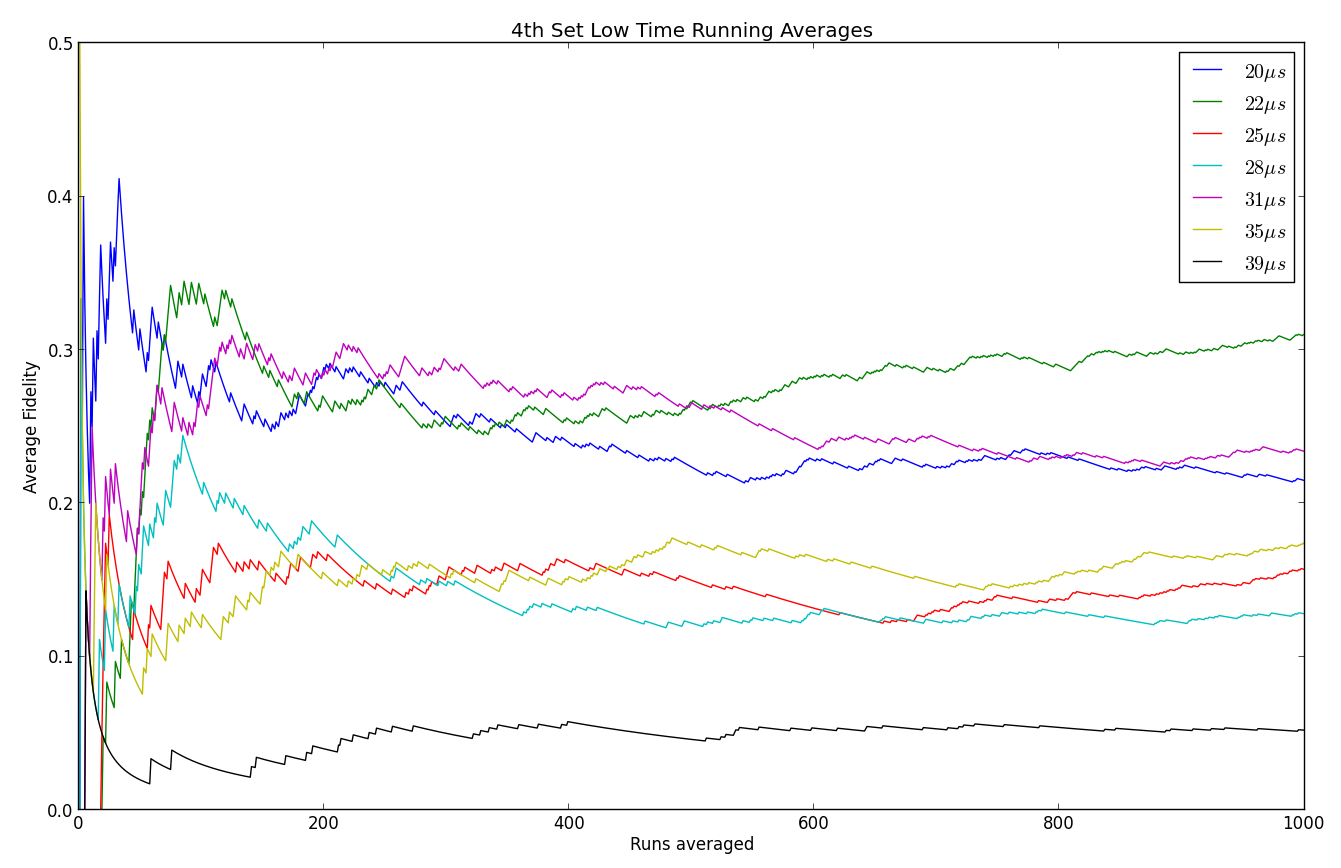
\includegraphics[bb= 0 0 1341 868]{img/4th_run_avg_low.png}
	}
	\caption[Running Fidelity Average]{Running average of the fidelity of the Hamiltonian ``6\_018'' for several short-time anneals, showing the change in fidelity with increasing read number.  The number of reads averaged over increases from zero to one thousand.  The rightmost edge of each data set shows the final fidelity estimate for that anneal time.  }
	\label{fig:running_avg}
\end{figure}
\section{Read noise}
First we examine the question of whether there is significant drift in the fidelity within a single run.  That is, does the probability of getting the ground state on any given read depend on the read number (the first read, second read etc.).  This question was examined on the Hamiltonian ``6\_018'' because the data collected on that particular Hamiltonian always consisted of at least 1000 reads per run.
Figure \ref{fig:running_avg} shows the running average of some short-time anneals from a single sweep of ``6\_018''.  If there is not significant read noise, we expect that the running average should flatten out and converge on the ``true'' fidelity after the appropriate number of reads.  For example, for a standard deviation $\sigma = \sqrt{np(1-p)}$ we expect that the running average should be within 5\% of the true fidelity after $\sim$ 200 reads.  Most of the anneal times appear to be reasonably flat past $\sim$ 500 reads, so the running averages appear to indicate to us that there isn't significant read noise (or at least, not nearly enough to be responsible for the short-time oscillations we saw in Chapter \ref{chap:prelim}).

The running average is a somewhat flawed quantity however, since it privileges earlier reads over later ones (since each read contributes like $1/N$ for $N$ reads already counted).  To remedy this we can also look at a rolling average of the fidelity as the reads come in.  Figure \ref{fig:rolling_avg} shows a rolling average of the fidelity for the same data as Figure \ref{fig:running_avg}.  Each point is the ground state fraction of the 100 reads around the labelled point; e.g. the value at point 500 is the number of ground states found from reads 450 to 550 over 100.  The rolling average has an advantage over the running average in that it does not prefer any part of the data set, but it can be harder to make out trends than in the running average.  It can be seen in the rolling average data that there does not appear to be a trend toward the fidelity being higher or lower in different segments of the run; e.g. the 22 $\mu$s run has highest fidelity in the nieghbourhood of read 600, while the 25 $\mu$s run has a minimum in the same location.

The combined results of the running and rolling averages would seem to indicate that intra-run errors, or errors occurring in the process of administering different reads, are not a significant contributor to the final observed fidelity for any given problem.

\begin{figure}
	\scalebox{0.35}{
		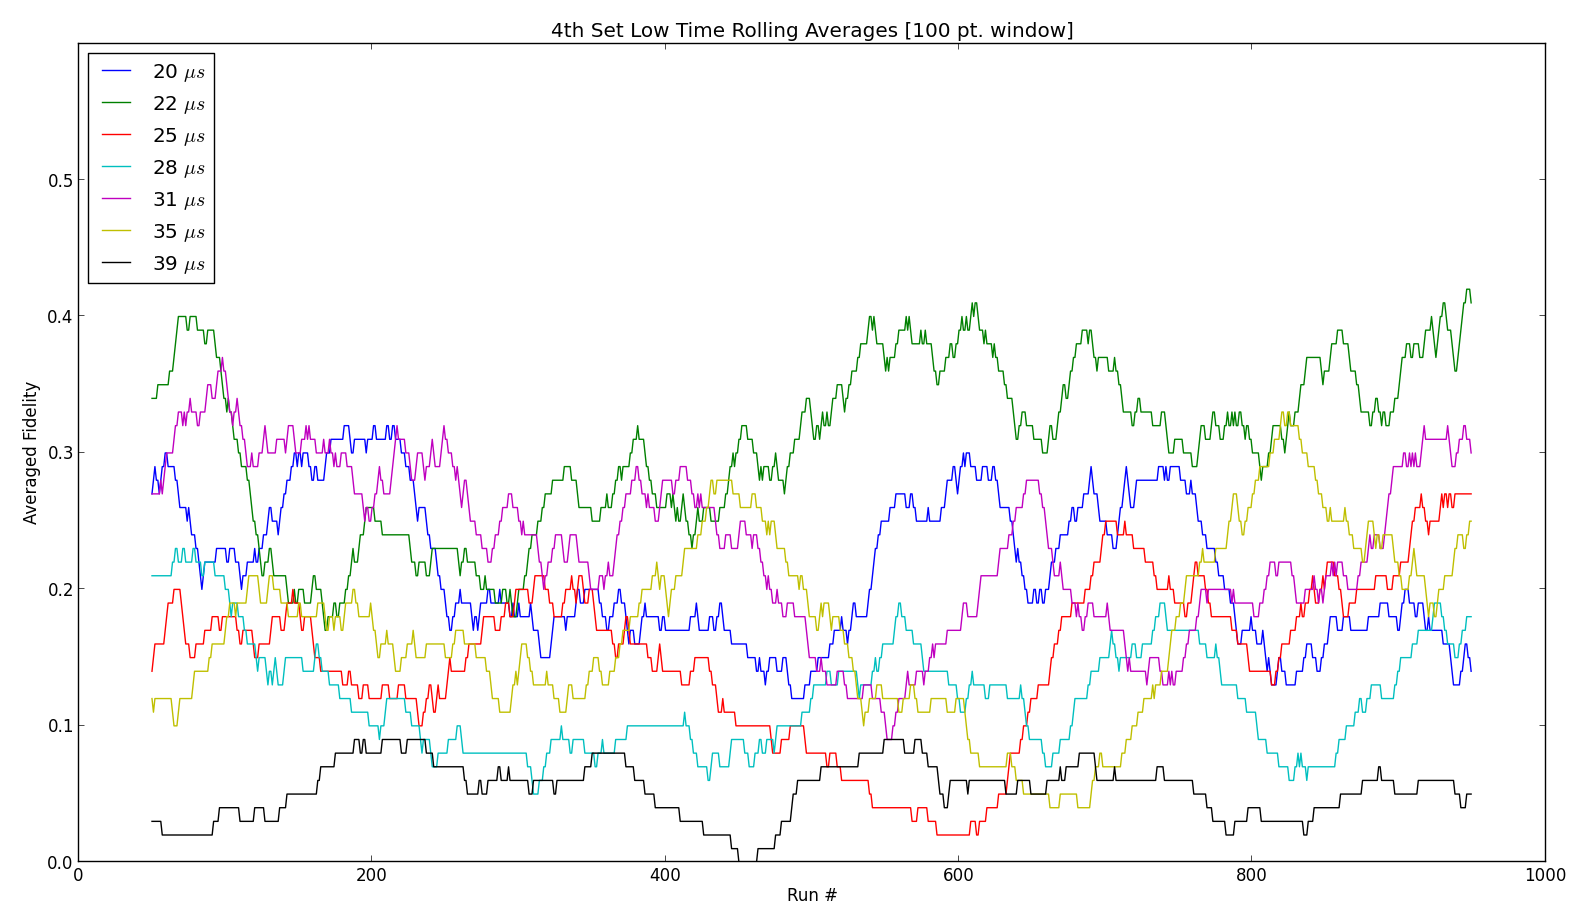
\includegraphics[bb=0 0 1582 917]{img/4th_run_roll_avg_low_100.png}
	}
	\caption[Rolling Fidelity Average]{Rolling average of the estimated fidelity for data collected from Hamiltonian ``6\_018'' at the seven shortest anneal times.  Each point is the average fidelity over a one hundred point window, e.g. the value at point 500 is the total number of times the ground state was measured between reads 450 and 550 divided by one hundred.}
	\label{fig:rolling_avg}
\end{figure}

\section{Short-time oscillations}
Looking to expand on the results of Chapter \ref{chap:prelim}, multiple sweeps of data were collected from a Hamiltonian labelled ``k44\_and''.  Figure \ref{fig:results_avg} shows the resulting fidelity estimates as a function of time.  This Hamiltonian not only occupies a single qubyte like ``k44'', but there is only one unique ground state.  These properties were chosen to attempt to minimize complicating factors.  Runs were carried out at annealing times from 20 $\mu$s to 20 ms as before.  Each run consisted of 100 reads, and 35 different runs were conducted at each anneal time.  Each fidelity estimate consists of a weighted average of each of the individual run estimates, weighted by the binomial error $\sigma$ for that run.
The error estimate at each anneal time is the standard deviation of the distribution of the individual run estimates.

Unlike in Chapter \ref{chap:prelim}, averaging over many runs at the same anneal time has managed to remove the short-time oscillations.  Figure \ref{fig:hist} shows a histogram of fidelities measured for ``k44\_and'' at an anneal time of 20 $\mu$s.  The Gaussian shape suggests that there are two effects going on: first, there is a value of the fidelity determined mainly by the quantum annealing (at the centre of the distribution) and second, that there is some noise applied over the fidelity from run to run.  The most likely source of this seems to be the programming error from imprecision of the physical couplings (see Sections \ref{sec:noise} and \ref{sec:coupling}).  If the noise in programming the couplings is high enough that if two adjacent couplings end up close enough together then the fidelity will drop because instead of the state we expect being the ground state and thus the most common, it will actually be some higher energy excited state and thus if the annealing is carried out successfully will have low probability of being found.  In the other scenario where two adjacent couplings are randomly bounced away from each other, it is entirely possible that in addition to the ground state being correctly encoded the gap is larger, thus increasing the fidelity.

\begin{figure}
	%includegraphics
	\caption[Averaged Anneal Results]{Fidelity vs anneal time with each data point averaged over multiple different runs.  Each run was used to estimate the fidelity independently as in Chapter \ref{chap:prelim}, with the final estimate the weighted average of each run.  The errorbars reflect the standard deviation of the distribution of estimates from each run.}
	\label{fig:results_avg}
\end{figure}

\begin{figure}
	%includegraphics
	\caption[Estimated Fidelity Histogram]{Histogram of the estimated fidelities for each run of the Hamiltonian ``k44\_and'' with an anneal time of 20 $\mu$s.  The shape appears roughly Gaussian, indicating that while there is a random factor in the fidelity that varies from run to run, there is still a central value that we take in this case to be roughly FIXME.}
	\label{fig:hist}
\end{figure}

\begin{figure}
	%includegraphics
	\caption[Fidelity Distribution vs. Time]{This figure shows the breadth of the distribution of estimated fidelities, i.e. the standard deviation $\sigma$ as a function of the annealing time for the Hamiltonian ``k44\_and''.  As the annealing time increases, the short-time oscillation effect observed in the preliminary results dies off and the distribution narrows.}
	\label{fig:std_time}
\end{figure}

Figure \ref{fig:std_time} shows the standard deviation of the fidelity estimates from evaluation of ``k44\_and'' as a function of the annealing time.  As we saw in the previous results, the large oscillations observed in the short-time fidelity die away as the annealing time increases.  This quantifies our earlier observation of the short-time oscillations: there are two regimes of the annealing, one below $\sim 500$ $\mu$s where the standard deviation is $\sim$ FIXME and one above $\sim 500$ $\mu$s where the standard deviation quickly drops down to FIXME.

This still does not explain \emph{why} the short-time oscillations do not persist into longer annealing times.  The above argument regarding overlap of the physical couplings applies just as well to annealing at longer times.

\section{Clone coupling value}
\label{sec:coupling}
As discussed in Sections \ref{sec:embed_algo} and \ref{sec:resolution}, while for an ideal machine maximizing the clone coupling value would ensure that adding clones did not alter the ground states of our problem Hamiltonians, the \texttt{VESUVIUS} machine can only implement 15 different clone coupling values.  In addition, these values must be evenly spaced.  If we were to use a clone coupling value of $-14$ in a problem Hamiltonian which natively had coupling values of $-2,-1,1,2$, this would result in compressing each of the positive and negative couplings into one machine value.  The machine only implements couplings of the form 
\begin{equation}
	\pm\frac{x}{7}, 1 \le x \le 7
\end{equation}
so the above example would result in a physically implemented Hamiltonian of $-1/7, -1/7, 1/7, 1/7$ in addition to the clone coupling of $-1$.  Most of the time this will result in a malformed Hamiltonian with incorrect ground states.

In addition to incorrect ground states, it is possible that the programming error in the machine is large enough to make the couplings $1/7$ and $2/7$ close enough to be likely to collide, whereas $1/7$ and $3/7$ could be far enough apart to be programmed correctly every time.  This could mean that even in scenarios where \texttt{VESUVIUS} has enough range to encode the problem Hamiltonian couplings correctly with a large clone coupling value we still don't want to do so.

This means that when selecting a clone coupling value we must balance these two competing factors, the desire to make the clone coupling as large as possible from a Hamiltonian correctness standpoint, and the desire to make it as small as possible from a machine resolution viewpoint.  The Hamiltonian correctness issue is correctness and knowable at the time the Hamiltonian is constructed; however in general to know whether a given clone coupling is large enough or not requires diagonalizing the Hamiltonian, and if this were possible then that would enable us to solve the initial computational problem directly.
The machine resolution problem is not necessarily the same from run to run; it could be that the compression of the problem Hamiltonian caused by the clone coupling value only makes it more likely for the machine to end up in an excited state.

To empirically examine the impact of the value of the clone coupling, the ``k44\_and'' Hamiltonian was embedded multiple different times with a clone coupling value ranging from -1 to -14 (from the smallest coupling in the problem Hamiltonian to twice the native resolution of the machine).  Figure \ref{fig:clone_coupling} shows the results of annealing these Hamiltonians from 20 $\mu$s to 20 ms.  Not only does fidelity increase as the clone coupling value is decreased, the short-time oscillations that we saw in Chapter \ref{chap:prelim} are removed.  At longer anneal times the difference in fidelity is reduced, and the same long-time drop in fidelities that was observed in other Hamiltonians continues.  This means that the mechanism for the long-time fidelity drop is not strongly impacted by the clone coupling value, which is what we would expect.

This provides more evidence that the short-time oscillations are caused by programming error in the \texttt{VESUVIUS} machine; if two couplings in the problem Hamiltonian are compressed together the correct ground states could still be formed in the resulting physical Hamiltonian if the couplings were randomly perturbed in the right directions, but this process would be random and differ greatly from run to run.

\begin{figure}
	%\includegraphics{}
	\caption[Variable Clone Coupling Fidelity]{The change in fidelity as the clone coupling value is scaled from -1 to -14.  The top view shows the scaling over the full time range 20 $\mu$s to 20 ms, while the bottom shows the same data zoomed in on the times 20 $\mu$s to 500 $\mu$s.  The fidelity increases with reducing clone coupling value, but using too small of a clone coupling value can result in incorrect ground states.}
	\label{fig:clone_coupling}
\end{figure}

\section{Size scaling}
The final property studied was the 
